\section{نمذجة الذراع الروبوتية باستخدام \LR{Simscape Multibody}}

\subsection{الغاية من نموذج \LR{Simscape}}

تم استخدام \LR{Simscape Multibody}  بهدف إنشاء نموذج محاكاة ميكانيكي للذراع الروبوتية داخل بيئة \\\LR{MATLAB/Simulink}. تعتمد هذه البيئة على تمثيل الأنظمة الميكانيكية متعددة الأجسام من خلال أجسام صلبة، ومفاصل، وقيود حركية، وعناصر قوى وعزوم، وحساسات قياس. وبذلك يمكن تمثيل الذراع الروبوتية كنظام مكوّن من عدة وصلات مترابطة، تتحرك فيما بينها وفق درجات الحرية المحددة بواسطة المفاصل.

تظهر أهمية هذا النموذج بشكل خاص عند التعامل مع الأنظمة الروبوتية متعددة درجات الحرية، لأن النموذج الرياضي الناتج عن الاشتقاق الديناميكي قد يصبح كبيرًا ومعقدًا بعد التعويض الكامل عن معاملات العطالة ومراكز الكتل وتحويلات الإحداثيات. فعلى الرغم من أن هذه المعادلات ضرورية لفهم السلوك الديناميكي للذراع، إلا أن حجمها الكبير يجعل التعامل معها مباشرة في المحاكاة أو التعديل أو الاختبار أمرًا غير عملي في كثير من الحالات.

تتمثل إحدى مشكلات المعادلات الضخمة في صعوبة قراءتها وتتبع حدودها الفيزيائية، إذ يصبح من الصعب تمييز مساهمة كل وصلة أو مفصل داخل المعادلة بعد التوسيع الرمزي الكامل. كما أن أي تعديل بسيط في التصميم، مثل تغيير كتلة وصلة أو موضع مركز كتلتها أو طول أحد الأجزاء، قد يتطلب إعادة حساب عدد كبير من الحدود. إضافة إلى ذلك، فإن استخدام المعادلات الموسعة مباشرة داخل نموذج تحكم أو محاكاة قد يزيد من التعقيد الحسابي ويجعل عملية التحقق من الأخطاء أكثر صعوبة.

لذلك تم الاعتماد على \LR{Simscape Multibody} كأداة مساعدة لبناء نموذج محاكاة عددي يعتمد على البنية الميكانيكية للذراع بدل التعامل المباشر مع جميع المعادلات الموسعة. فالنموذج في \LR{Simscape} لا يتطلب كتابة معادلات الحركة يدويًا بشكلها الكامل، بل يتم بناء النظام من عناصر ميكانيكية مثل الأجسام والمفاصل، ثم تقوم بيئة المحاكاة بصياغة وحل معادلات الحركة للنظام الكامل.

وبناءً على ذلك، فإن الهدف من نموذج \LR{Simscape} في هذا العمل هو توفير تمثيل محاكاة قريب من البنية الميكانيكية الفعلية للذراع، بحيث يمكن دراسة حركة المفاصل واستجابة النظام داخل بيئة \LR{Simulink}. كما يسمح هذا النموذج لاحقًا بربطه مع نماذج التشغيل أو خوارزميات التحكم، دون الحاجة إلى إدخال المعادلات الديناميكية الطويلة يدويًا داخل نموذج المحاكاة.







\subsection{تصدير نموذج \LR{SolidWorks}}

بعد تجهيز نموذج الذراع الروبوتية على شكل تجميع ميكانيكي داخل برنامج \LR{SolidWorks}، تم التحقق من الشكل العام للذراع وترتيب الوصلات والمفاصل كما هو واضح في الشكل \ref{fig:model_in_solid}.

\begin{figure}[H]
\centering
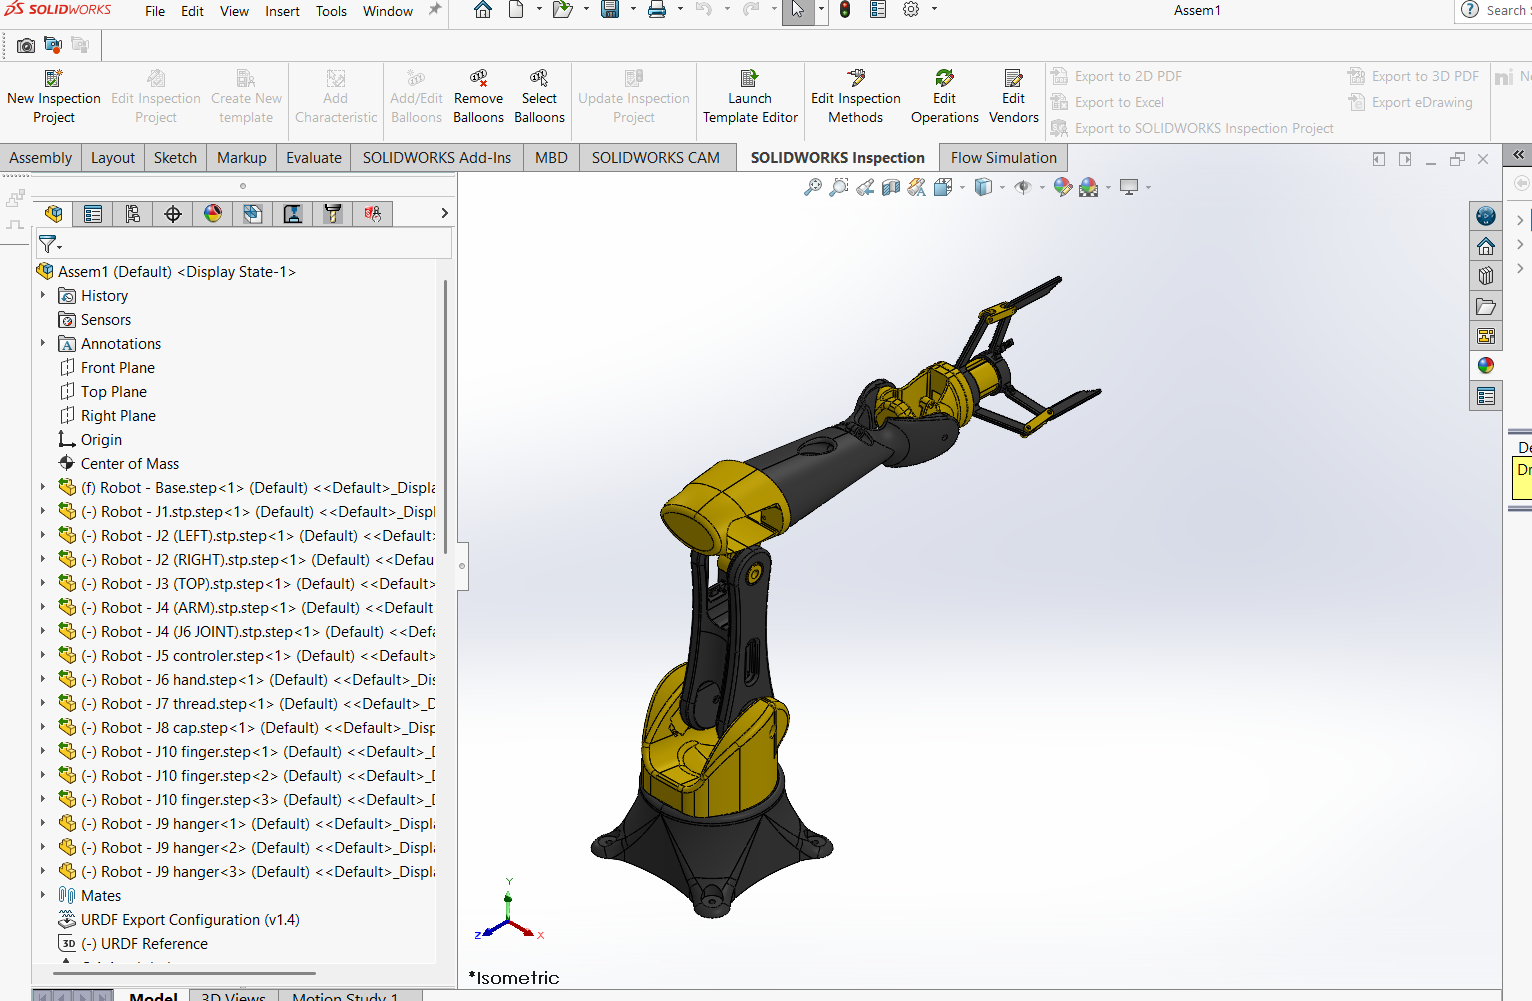
\includegraphics[width=0.85\textwidth]{resources/images/Model_in_solid}
\caption{\centering{نموذج الذراع الروبوتية داخل برنامج \LR{SolidWorks}}}
\label{fig:model_in_solid}
\end{figure}

بعد التأكد من اكتمال نموذج التجميع داخل \LR{SolidWorks}، تم الانتقال إلى مرحلة تصدير النموذج إلى بيئة \LR{Simscape} \LR{Multibody}. وتتم عملية التصدير من خلال المسار التالي داخل برنامج \LR{SolidWorks}:

\begin{center}
\begin{LTR}
Tools $\Rightarrow$ Simscape Multibody Link $\Rightarrow$ Export $\Rightarrow$ Simscape Multibody
\end{LTR}
\end{center}
كما هو واضح في الشكل \ref{fig:export_simscape}.

\begin{figure}[H]
\centering
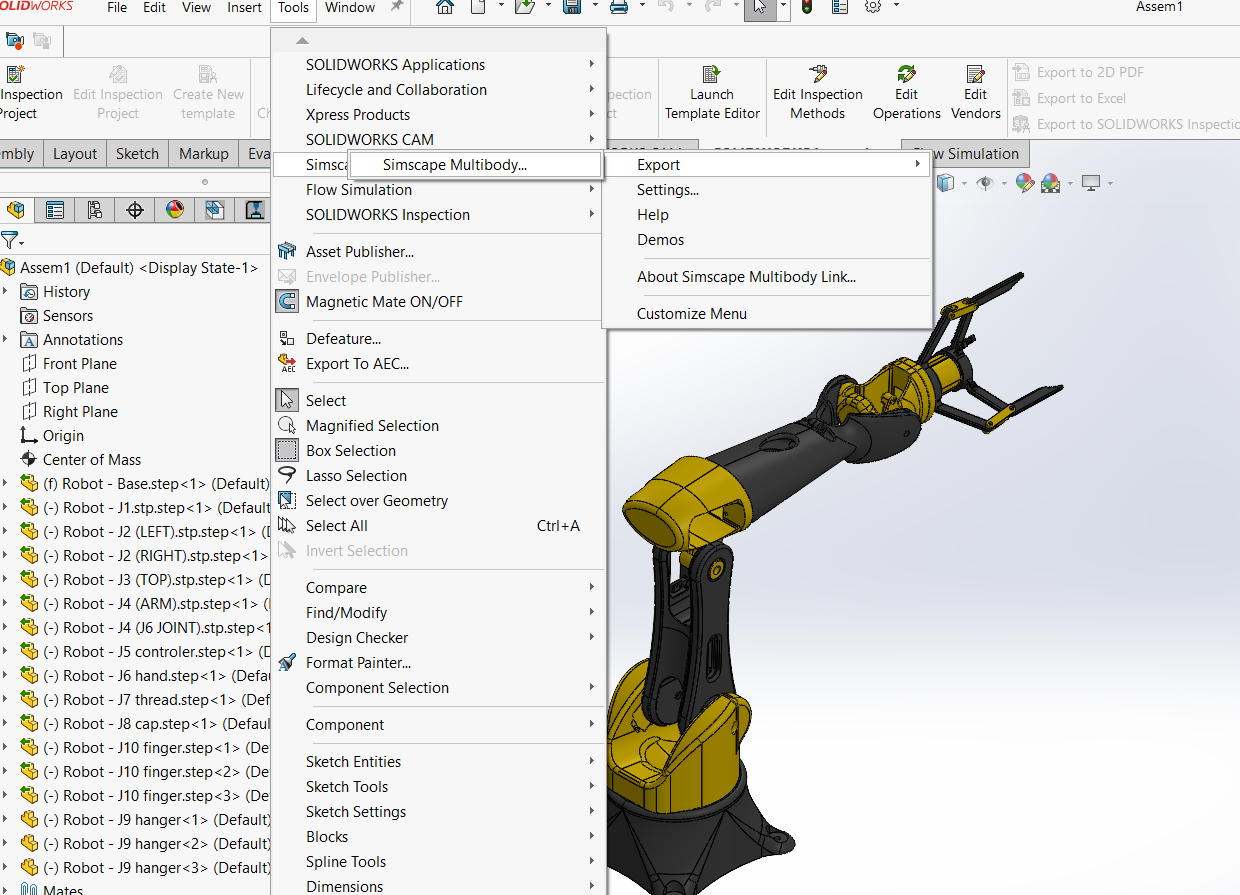
\includegraphics[width=0.85\textwidth]{resources/images/export_simscape}
\caption{\centering{خطوة تصدير نموذج \LR{SolidWorks} إلى \LR{Simscape} \LR{Multibody}}}
\label{fig:export_simscape}
\end{figure}

بعد اختيار أمر التصدير، يقوم برنامج \LR{SolidWorks} بإنشاء ملف بصيغة \LR{XML} يحتوي على وصف بنية التجميع الميكانيكي، إضافة إلى ملفات هندسية مرافقة تمثل أشكال الأجزاء. وتستخدم هذه الملفات لاحقًا داخل بيئة \LR{MATLAB}/\LR{Simulink} لإنشاء نموذج محاكاة مكافئ للذراع الروبوتية في \LR{Simscape} \LR{Multibody}.

تمثل هذه الخطوة مرحلة الربط بين التصميم الميكانيكي والمحاكاة، إذ يتم تحويل نموذج الذراع من تجميع هندسي داخل \LR{SolidWorks} إلى نموذج قابل للاستيراد والبناء داخل \LR{Simscape}. وتبقى دقة النموذج الناتج مرتبطة بصحة نموذج التجميع الأصلي، من حيث ترتيب الأجزاء، وتعريف المواد والكتل، ومواضع الوصلات والمفاصل.



\subsection{بناء نموذج المحاكاة في \LR{Simscape}}

بعد تصدير نموذج الذراع من برنامج \LR{SolidWorks}، تم الانتقال إلى بيئة \LR{MATLAB} من أجل استيراد ملف النموذج الناتج. تم ذلك باستخدام الأمر \LR{smimport}، حيث يتم استدعاء ملف \LR{XML} الناتج عن عملية التصدير كما يلي:

\begin{center}
\LR{smimport("Assem1.xml")}
\end{center}

يقوم هذا الأمر بقراءة ملف \LR{XML} الذي يحتوي على وصف بنية التجميع الميكانيكي، ثم يعمل على إنشاء نموذج \LR{Simulink} يحتوي على عناصر \LR{Simscape} \LR{Multibody} الموافقة لأجزاء الذراع. وبهذه الطريقة يتم تحويل النموذج القادم من \LR{SolidWorks} إلى نموذج محاكاة قابل للتشغيل داخل بيئة \LR{MATLAB}/\LR{Simulink}، كما هو واضح في الشكل \ref{fig:export_XML}.

\begin{figure}[H]
\centering
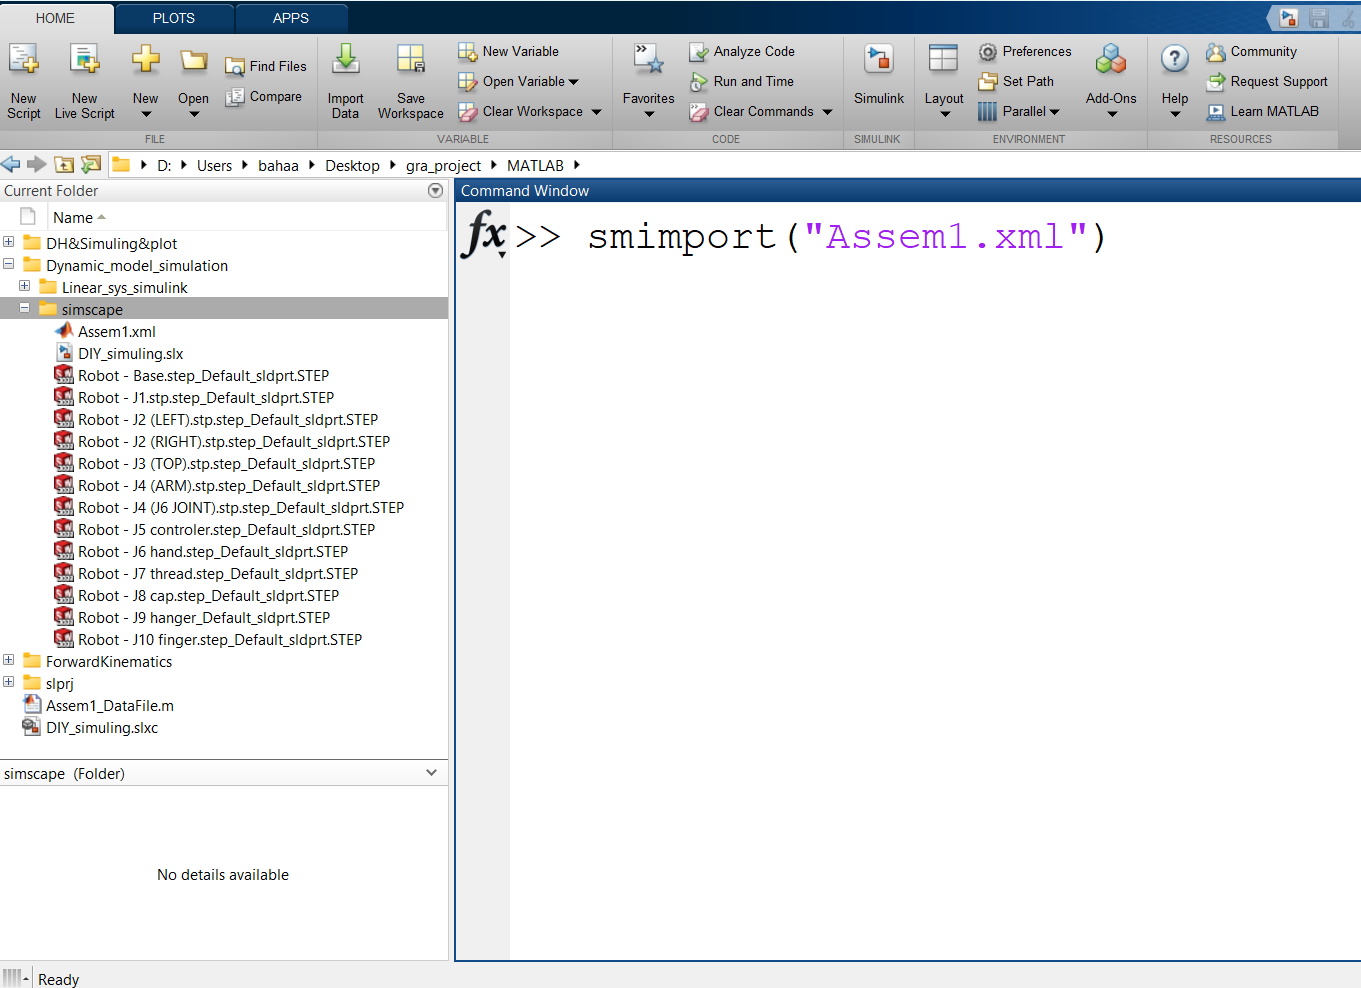
\includegraphics[width=0.85\textwidth]{resources/images/export_XML}
\caption{\centering{استيراد ملف \LR{XML} داخل \LR{MATLAB} باستخدام الأمر \LR{smimport}}}
\label{fig:export_XML}
\end{figure}

بعد تنفيذ الأمر السابق، يتم توليد نموذج جديد داخل \LR{Simulink} يمثل الذراع الروبوتية على شكل منظومة ميكانيكية متعددة الأجسام. يحتوي هذا النموذج على الأجسام الصلبة الخاصة بالوصلات، والإطارات المرجعية، والمفاصل التي تربط أجزاء الذراع مع بعضها. كما يمكن ملاحظة أن النموذج الناتج يحافظ على تقسيم أجزاء الذراع، بما في ذلك الجزء الطرفي \LR{End Effector} كما هو واضح في الشكل \ref{fig:end_effector}، إضافة إلى النموذج الكامل للذراع كما هو واضح في الشكل \ref{fig:robot_plant}.

\begin{figure}[H]
\centering
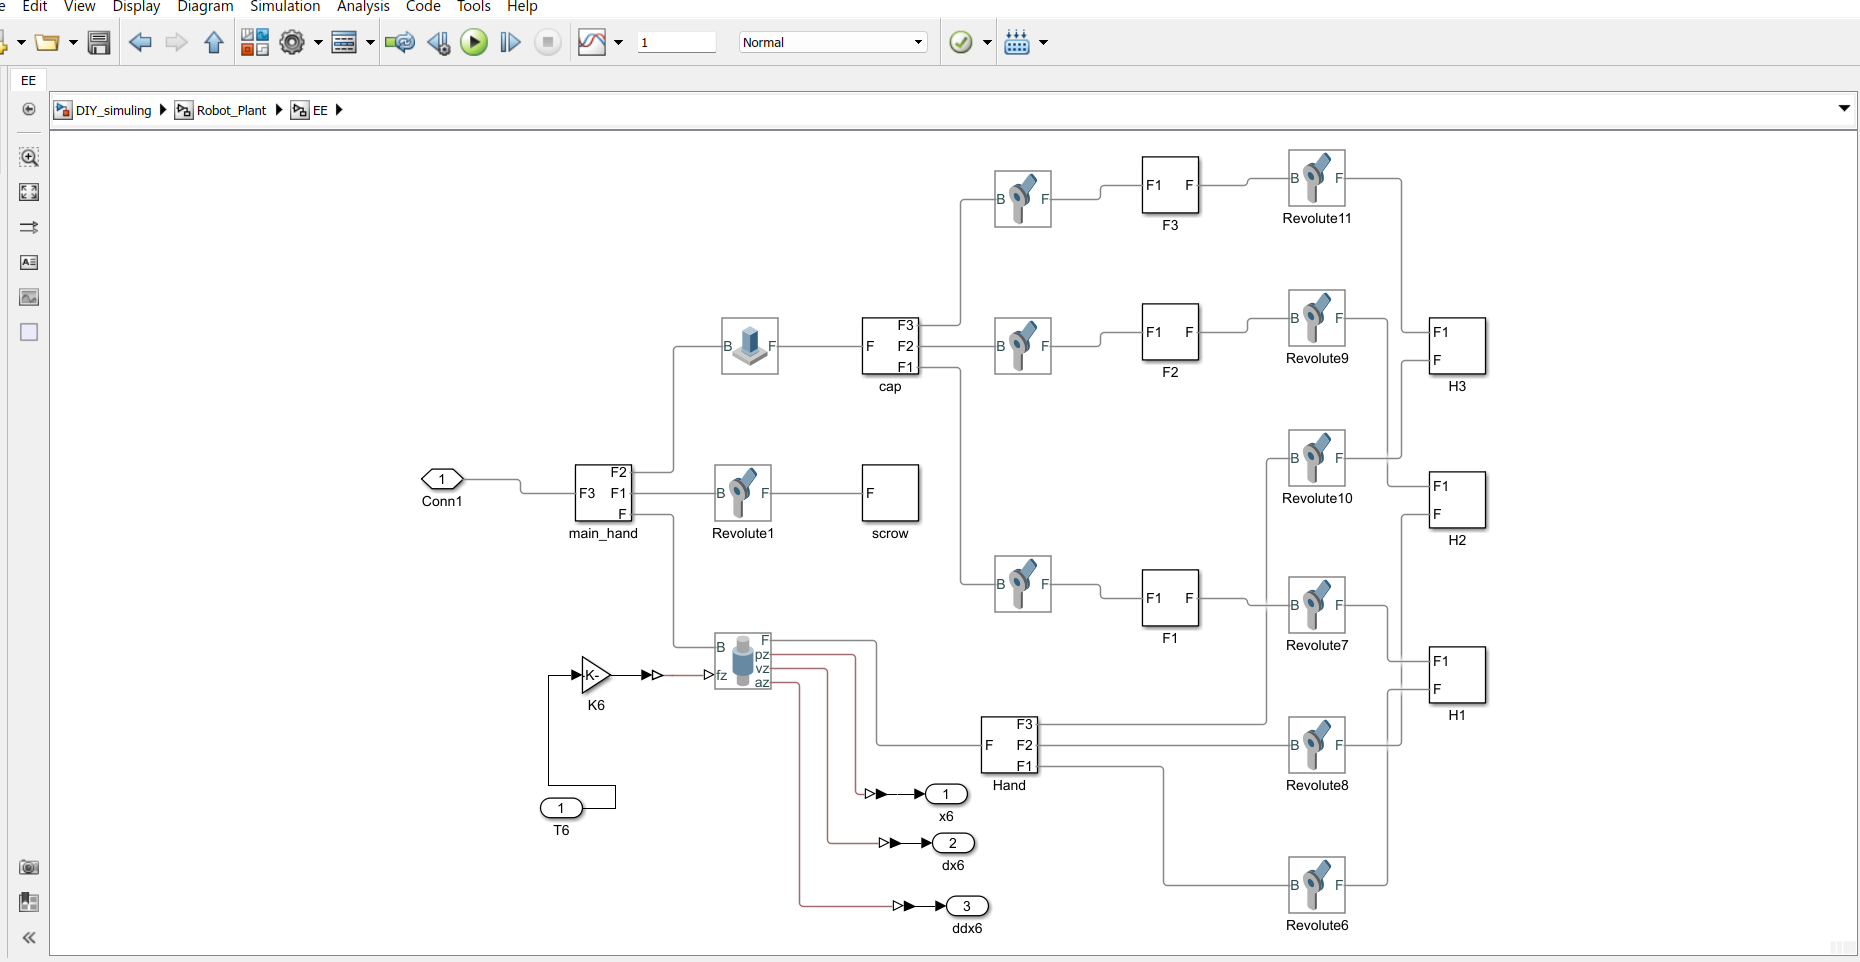
\includegraphics[width=0.85\textwidth]{resources/images/end_effector}
\caption{\centering{نموذج الجزء الطرفي \LR{End Effector} بعد الاستيراد إلى \LR{Simscape}}}
\label{fig:end_effector}
\end{figure}

\begin{figure}[H]
\centering
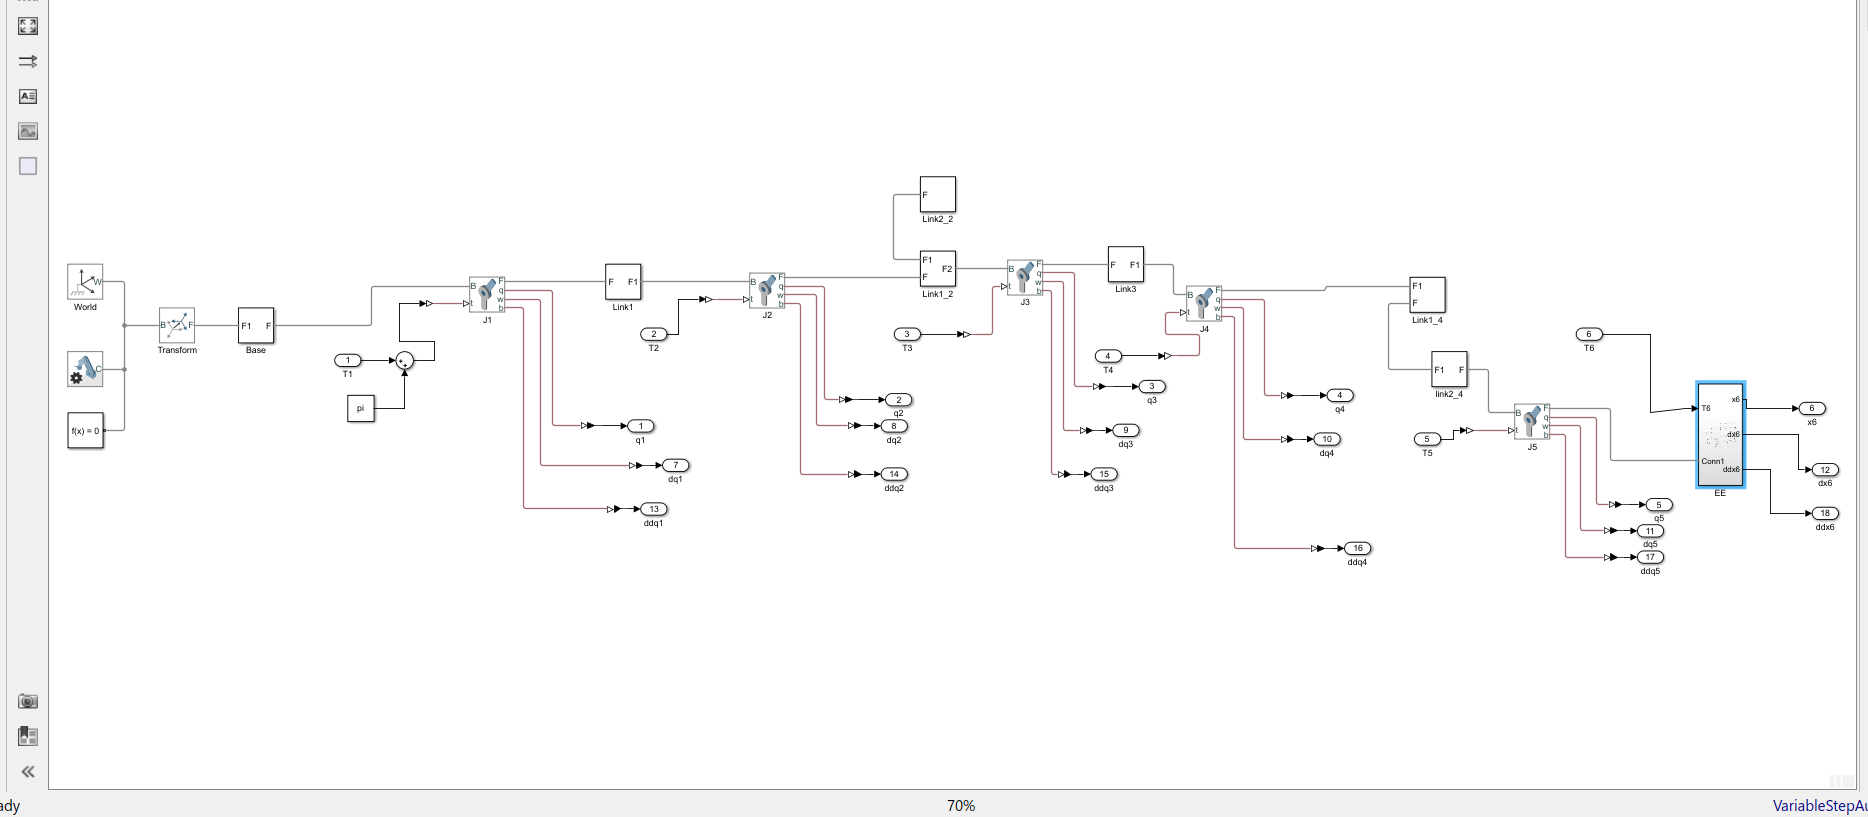
\includegraphics[width=0.95\textwidth]{resources/images/robot_plant}
\caption{\centering{النموذج الكامل للذراع الروبوتية داخل بيئة \LR{Simscape} \LR{Multibody}}}
\label{fig:robot_plant}
\end{figure}

وبذلك يصبح النموذج جاهزًا للتعديل والمحاكاة داخل بيئة \LR{Simscape} \LR{Multibody}، حيث يمكن لاحقًا ضبط مداخل المفاصل، وإضافة عناصر القياس، وربط النموذج مع بيئة \LR{Simulink}.









\subsection{استخدام النموذج في بيئة \LR{Simulink}}

بعد بناء نموذج الذراع الروبوتية داخل بيئة \LR{Simscape} \LR{Multibody}، أصبح بالإمكان تشغيل النموذج داخل \LR{Simulink} ومراقبة استجابة الذراع أثناء المحاكاة. يتيح هذا النموذج تمثيل الذراع كنظام ميكانيكي قابل للتشغيل، حيث يمكن متابعة وضعية الوصلات والمفاصل ضمن نافذة العرض ثلاثية الأبعاد الخاصة بـ \LR{Simscape}.

يساعد تشغيل النموذج داخل \LR{Simulink} على التأكد من أن عملية الاستيراد من \LR{SolidWorks} تمت بشكل صحيح، وأن أجزاء الذراع مترابطة كما هو متوقع داخل نموذج المحاكاة. كما يسمح هذا النموذج لاحقًا بإضافة مداخل للمفاصل، مثل الزوايا أو العزوم، وربطه مع أنظمة التشغيل أو خوارزميات التحكم المراد اختبارها.

وعند تشغيل المحاكاة، يظهر النموذج ثلاثي الأبعاد للذراع الروبوتية داخل نافذة العرض الخاصة بـ \LR{Simscape} \LR{Multibody}. يوضح الشكل \ref{fig:simuling_DIY} شكل الذراع أثناء تشغيل النموذج داخل بيئة المحاكاة.

\begin{figure}[H]
\centering
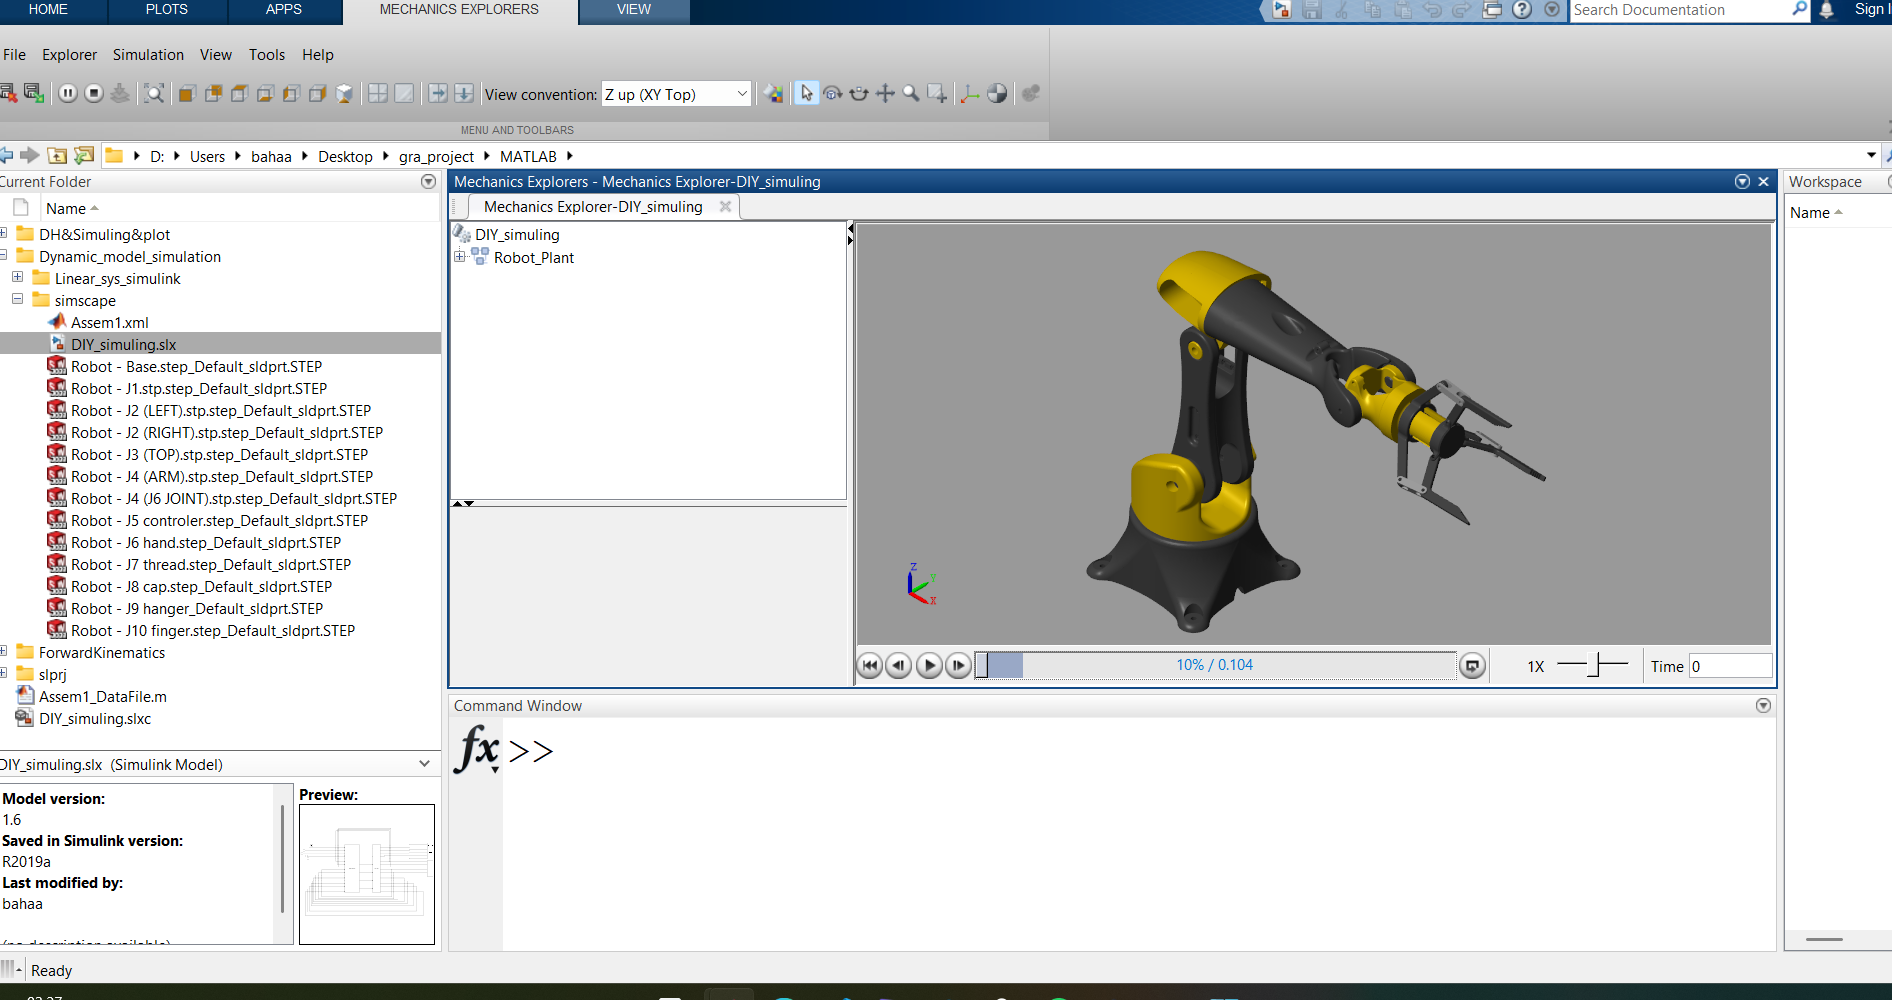
\includegraphics[width=0.90\textwidth]{resources/images/simuling_DIY}
\caption{\centering{ الذراع  أثناء تشغيل المحاكاة في \LR{Simscape} \LR{Multibody}}}
\label{fig:simuling_DIY}
\end{figure}

يوضح الشكل أن النموذج الناتج أصبح قابلًا للتشغيل داخل بيئة المحاكاة، وأن الذراع تظهر بشكل ثلاثي الأبعاد مع إمكانية متابعة وضعيات الوصلات والمفاصل أثناء التشغيل. وبذلك يمكن اعتبار نموذج \LR{Simscape} \LR{Multibody} هو النموذج الميكانيكي المستخدم داخل \LR{Simulink} لدراسة حركة الذراع واختبار سلوكها قبل الانتقال إلى مرحلة التحكم أو التطبيق العملي.

\subsection{حدود دقة نموذج المحاكاة في \LR{Simscape}}


على الرغم من أن نموذج \LR{Simscape} \LR{Multibody} يوفر تمثيلًا عمليًا ومفيدًا للذراع الروبوتية داخل بيئة المحاكاة، إلا أن دقة هذا النموذج تبقى مرتبطة بعدة عوامل وافتراضات. فالنموذج الناتج يعتمد بشكل مباشر على دقة التصميم الميكانيكي الأصلي في \LR{SolidWorks}، من حيث أبعاد الوصلات، ومواضع المفاصل، وترتيب الأجزاء داخل التجميع.

كما تعتمد الخصائص الفيزيائية المنقولة إلى نموذج المحاكاة، مثل الكتل ومراكز الكتل وعزوم العطالة، على صحة تعريف المواد والكثافات داخل نموذج \LR{SolidWorks}. لذلك فإن أي خطأ في تعريف مادة أحد الأجزاء أو في موضع مركز كتلته قد يؤدي إلى اختلاف في سلوك النموذج أثناء المحاكاة.

ومن جهة أخرى، فإن النموذج المستورد إلى \LR{Simscape} يمثل بصورة أساسية البنية الميكانيكية للذراع، أي الوصلات والمفاصل والعلاقات الحركية بينها. أما خصائص المشغلات الحقيقية، مثل حدود العزم، وحدود السرعة، والتأخير الزمني، والاحتكاك الداخلي، فلا تكون ممثلة بشكل كامل ما لم تتم إضافتها يدويًا إلى نموذج المحاكاة.

كذلك فإن بعض التأثيرات الموجودة في النظام الحقيقي، مثل الاحتكاك في المفاصل، والخلوص الميكانيكي، ومرونة الأجزاء، قد لا تظهر في النموذج إلا إذا تم تمثيلها بعناصر إضافية داخل \LR{Simulink}/\LR{Simscape}. لذلك يجب التعامل مع نتائج المحاكاة على أنها تقريب لسلوك الذراع الحقيقي، وليست بديلًا كاملًا عن الاختبار العملي.

وبناءً على ذلك، فإن نموذج \LR{Simscape} المستخدم في هذا العمل يعد أداة مناسبة لدراسة الحركة العامة للذراع، والتحقق من بنية النموذج، واختبار السلوك المبدئي قبل التطبيق العملي. ومع ذلك، فإن الوصول إلى تمثيل أكثر دقة يتطلب إضافة نماذج تفصيلية للمحركات، والاحتكاك، وحدود التشغيل، ثم مقارنة نتائج المحاكاة مع القياسات العملية عند توفرها.